\documentclass[UTF8,a4paper,11pt]{ctexart}
\usepackage[margin=20mm,includehead,headheight=17pt,headsep=7mm]{geometry}
\usepackage{fontspec,amsmath,amssymb,booktabs,array,graphicx,xcolor,hyperref,fancyhdr,enumitem}
\setmainfont{Latin Modern Roman}
\setsansfont{Latin Modern Sans}
\setCJKmainfont{Noto Serif CJK SC}
\setCJKsansfont{Noto Sans CJK SC}
\setmonofont{JuliaMono-Regular.ttf}[Path=/root/.agents/skills/make-pdf/assets/fonts/]
\definecolor{ink}{HTML}{18334F}
\definecolor{accent}{HTML}{265CA6}
\definecolor{light}{HTML}{EEF3F9}
\hypersetup{colorlinks=true,linkcolor=accent,urlcolor=accent,pdftitle={命题6.20：固定目标版本的谱反例与Adams图}}
\pagestyle{fancy}
\fancyhf{}
\fancyhead[L]{\small\textsf{Proposition 6.20 · 审阅材料}}
\fancyhead[R]{\small 固定目标与非提升首项}
\fancyfoot[C]{\small\thepage}
\setlength{\parindent}{0pt}
\setlength{\parskip}{5pt}
\setlist[itemize]{nosep,leftmargin=1.5em}
\setlength{\tabcolsep}{6pt}
\renewcommand{\arraystretch}{1.2}
\newcommand{\ZZ}{\mathbb Z}
\newcommand{\FF}{\mathbb F_2}
\newcommand{\AF}{\operatorname{AF}}
\newcommand{\Ext}{\operatorname{Ext}}
\newcommand{\sect}[1]{\vspace{3pt}{\large\bfseries\sffamily\color{ink}#1}\par}
\begin{document}
{\LARGE\bfseries\sffamily\color{ink}命题 6.20：固定目标版本的谱反例}

{\large Adams 图、有限 \(\lambda\) 商与具体计算}\hfill 2026-10-17

\colorbox{light}{\parbox{\dimexpr\linewidth-2\fboxsep\relax}{
\textbf{请核对的版本。} 固定原目标 \(y\)、由分次推出 \(b=0\)，同时保留
\(x'\in Z_{\mathrm{early}}\setminus Z_{\mathrm{late}}\) 的非提升首项条件。
下例针对这个版本的\textbf{必要方向}；不否定首段合法域自然性，也不替未明确目标关联的印刷一般 \(b\) 版本作出解释。}}

\sect{1. 谱、映射与合法参数}
令 \(E=H\ZZ_2^\wedge\)、\(M=H(\ZZ/16)\)，取标准三角
\[
 E\xrightarrow{16}E\longrightarrow M\xrightarrow{\delta}\Sigma E.
\]
定义实际谱与映射
\[
\begin{split}
X&=\Sigma E_x\oplus\Sigma E_u\oplus M,\qquad
Y=\Sigma E_z\oplus\Sigma E_{y_0},\\
f|_{\Sigma E_x}&=8\,i_{y_0},\qquad
f|_{\Sigma E_u}=2\,i_z,\qquad f|_M=(\delta,2\delta).
\end{split}
\]
各谱均为 2 完备、connective、逐度 mod-2 finite type。由于 \(\delta\) 在 mod-2 同调上非零，
\(\AF(f)=e(f)=0\)。取
\[
 (s,t)=(0,1),\quad n=3,\quad r'=5,\quad r=7,\qquad
 y=h_0^3y_0\in\Ext^{3,4}(Y).
\]
\(x\in\Ext^{0,1}(X)\) 为第一个悬挂 \(E\) 的首类；\(x,y\) 都永久。
早页长度合法：\(0\le3\le5-2\)。

\sect{2. 从实际三角得到有限坐标}
记 \(N=\nu E\)、\(Q_q(T)=T/\lambda^q\)。归一化三角为
\[
 \Sigma^{0,1}N\xrightarrow{\widehat{16}}N
 \longrightarrow\nu M\xrightarrow{\nu\delta}\Sigma^{1,1}N.
\]
在本计算的自由 \(h_0\) 塔上，\(\lambda h_0=2\)，
\(\widehat{16}=16/\lambda=\lambda^3h_0^4\)。在 weight 1 的源基底 \(1\) 与靶基底
\(h_0\) 上，\(\widehat{16}\) 的系数为 \textbf{8}。固定 stem 1、weight 1 的正合列给出
\[
0\longrightarrow\pi_{1,1}Q_q(\nu M)
\xrightarrow{\nu\delta}\ZZ/2^q
\xrightarrow{8}h_0\,\ZZ/2^q.
\]
因此指定连接坐标的像为
\[
K_q=\ker(8:\ZZ/2^q\to\ZZ/2^q),\qquad
K_4=2\ZZ/16,\quad K_6=8\ZZ/64.
\]
\(\rho:Q_6\to Q_4\) 与此三角自然交换，故坐标中为模 16 约化。各坐标的 Adams
滤过由 \(2^a\) 整除性给出；\(M\) 分量取与 \(K_q\) 的交。
同一实际 \(\nu f/\lambda^q\) 为
\[
\boxed{\quad f_q(\alpha,\beta,c)=(2\beta+c,\;8\alpha+2c),\quad
(\alpha,\beta,c)\in(\ZZ/2^q)^2\oplus K_q.\quad}
\]
靶坐标依次为 \((z,y_0)\)，原 synthetic 目标 \(\lambda^3h_0^3y_0\) 对应 \((0,8)\)。

\newpage
\sect{3. 经典 \(\mathrm{HF}_2\)-Adams 图}
\begin{center}
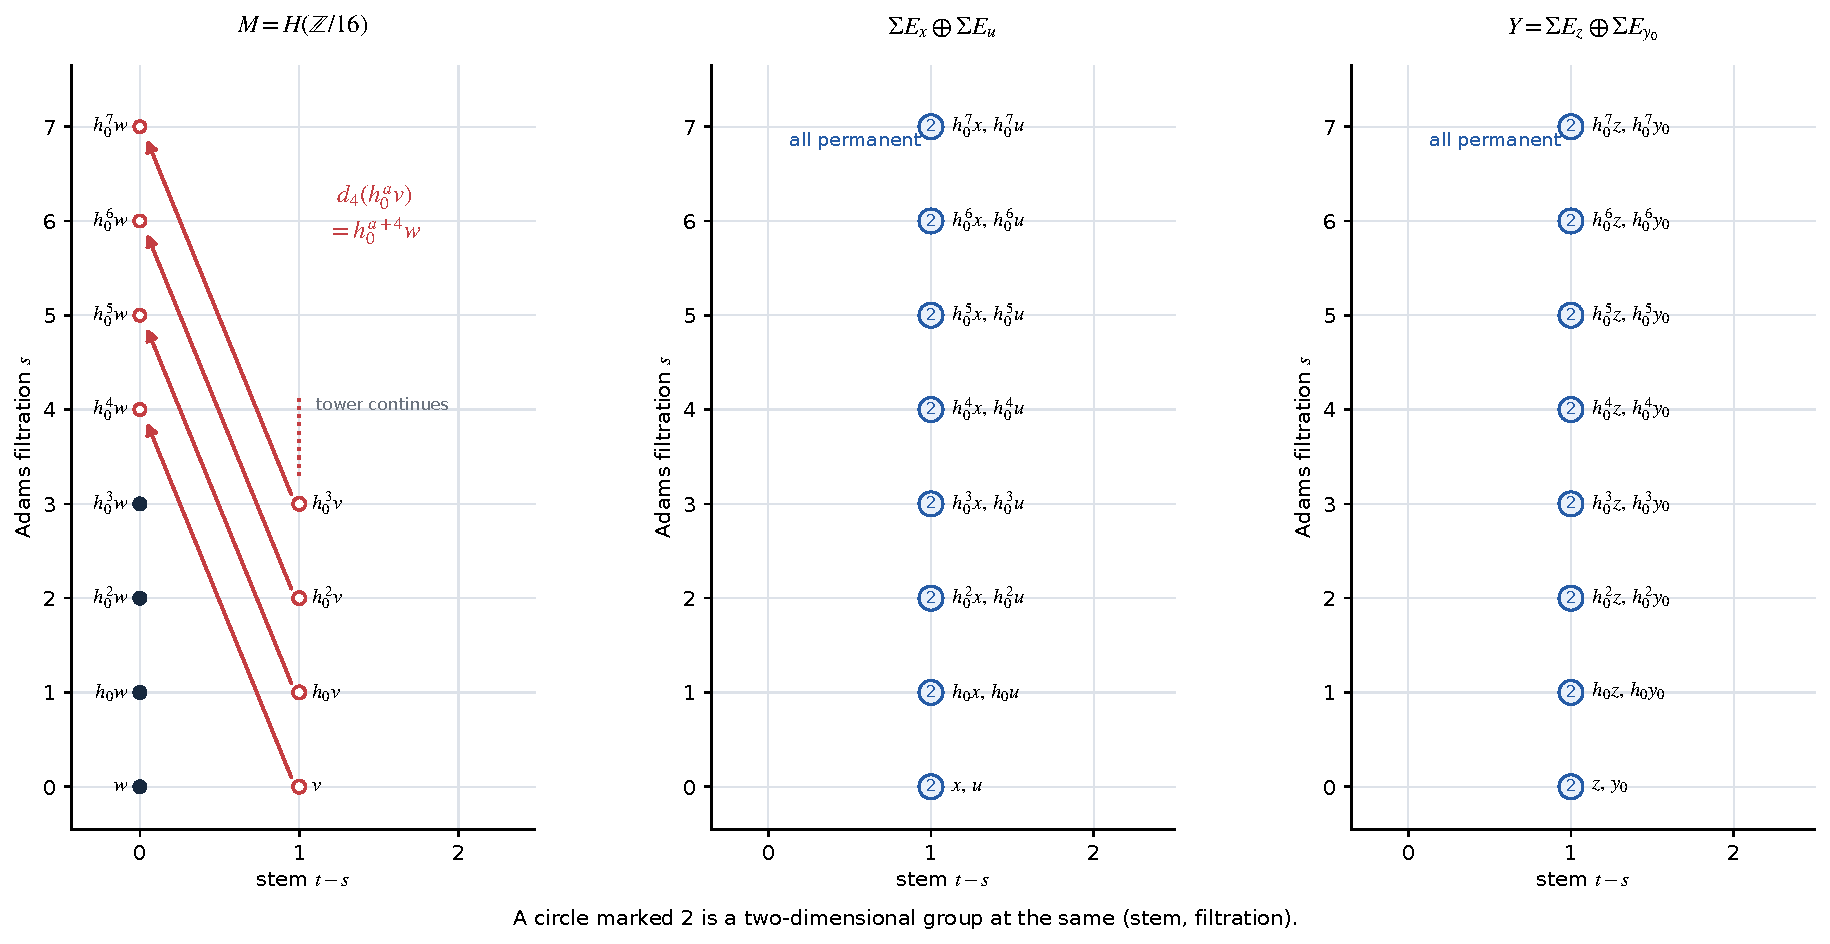
\includegraphics[width=\linewidth]{classical-adams.pdf}
\end{center}
横轴是真正的 stem \(t-s\)，纵轴是 Adams 滤过 \(s\)。标有“2”的圆表示同一个
双分次中的二维空间，并不表示两个不同 stem。
左图展示 \(M\) 的 \(E_2\) 两塔和全部平移的 \(d_4\) 模式：
\[
\Ext(M)=\FF[h_0]\{w,v\},\qquad |w|=(0,0),\quad |v|=(0,1),
\qquad d_4(h_0^av)=h_0^{a+4}w.
\]
实心 \(w,h_0w,h_0^2w,h_0^3w\) 为经典永久类；空心红点为 \(d_4\) 的源或靶。
\(\Sigma E_x,\Sigma E_u,Y\) 的各条塔均永久。

\sect{4. 为何有限商中会出现不可提升的 \(v\) 首项}
经典 \(v\) 塔被 \(d_4\) 杀掉，并不意味着所有有限 \(\lambda\) 商中的对应带权类都消失。
在固定 stem 1、weight 1 的有效条带 \(0\le a<q\) 内，
\[
\lambda^a h_0^av\in E_\infty(Q_q\nu M)
\quad\Longleftrightarrow\quad
h_0^av\in Z_{q-a}
\quad\Longleftrightarrow\quad a+3\ge q.
\]
这里 \(x,u,v,z,y_0\) 的经典 stem 都是 1；每个 \(h_0\) 增加一次滤过，
每个 \(\lambda\) 降低一次 weight。
\begin{center}
\begin{tabular}{ccll}
\toprule
源滤过 \(a\)&早页 \(q=4\)&晚页 \(q=6\)&结论\\
\midrule
1&\(\lambda h_0v\) 存活&对应首项不存活&不可提升\\
2&\(\lambda^2h_0^2v\) 存活&对应首项不存活&不可提升\\
3&\(\lambda^3h_0^3v\) 存活&对应首项存活&可以提升\\
\bottomrule
\end{tabular}
\end{center}
所以原文允许的 \(1\le a\le n-e(f)=3\) 中，
\[
Z_{4-a}^{a,1+a}(X)\setminus Z_{6-a}^{a,1+a}(X)
\]
只在 \(a=1,2\) 非空，且首项必须含非零 \(v\) 分量。
\(x,u\) 的永久塔全部可提升。这里同一边界分母包含于晚页 cycles，
因此更换模边界同余代表不能掩盖真正的非提升性。

\newpage
\sect{5. 固定 weight 1 的有限商 \(E_\infty\) 与 ESS 图}
\begin{center}
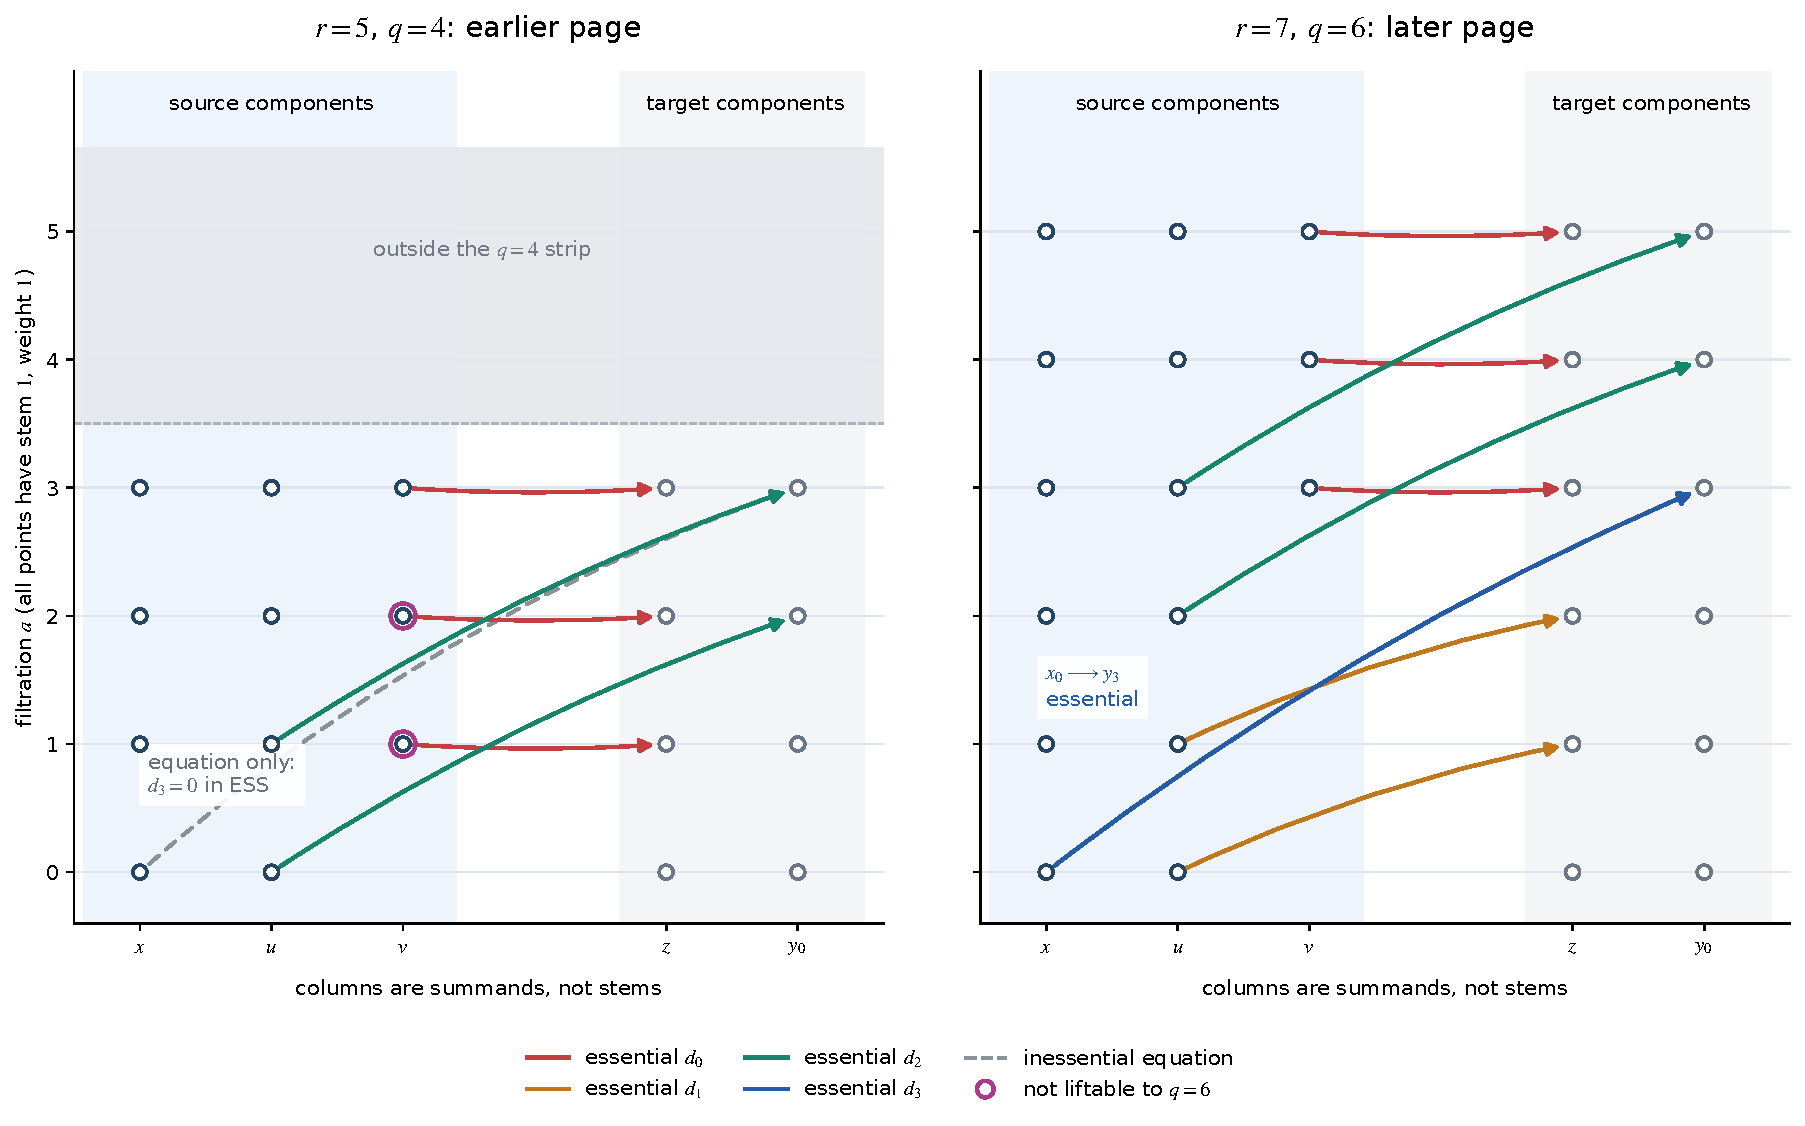
\includegraphics[width=\linewidth]{finite-ess.pdf}
\end{center}
\textbf{此图横轴按直和分量排列，不是 stem 轴。}
所有点的经典 stem 都为 1，synthetic weight 都为 1；纵轴为滤过 \(a\)。
在 \(x,u,v,z,y_0\) 列，第 \(a\) 行表示相应的 \(\lambda^a h_0^a\) 类。
紫色外圈标出早页不能提升到 \(q=6\) 的两个首项。

彩色实线是这条带中的\textbf{非零 ESS 微分}：
\begin{center}\small
\begin{tabular}{cll}
\toprule
页&非零微分&范围\\
\midrule
\(q=4\)&\(d_0(v_a)=z_a\)&\(a=1,2,3\)\\
&\(d_2(u_a)=y_{a+2}\)&\(a=0,1\)\\
\midrule
\(q=6\)&\(d_0(v_a)=z_a\)&\(a=3,4,5\)\\
&\(d_1(u_a)=z_{a+1}\)&\(a=0,1\)\\
&\(d_2(u_a)=y_{a+2}\)&\(a=2,3\)\\
&\(d_3(x_0)=y_3\)&\\
\bottomrule
\end{tabular}
\end{center}
表中的下标为滤过，不是经典元素的新命名。\(d_2\) 的实际源代表可取
\((0,2^a,-2^{a+1})\)，其像为 \((0,-2^{a+2})\)；关联分次在 \(\FF\) 上，
负号不影响图上的非零类。

\textbf{灰虚线不是非零 ESS 微分。} 在早页，\(y_3\) 已是 \(d_2(u_1)\) 的边界，
所以原 \(x_0\) 到 \(y_3\) 的长度 3 扩张方程为 inessential：
它在 ESS 第 3 页等于零。晚页同一 \(d_3(x_0)=y_3\) 才是 essential。

\newpage
\sect{6. essential / inessential 的完整不定性计算}
\textbf{晚页 \(r=7\)，即 \(q=6\)。}
源 \((1,0,0)\) 映到 \((0,8)\)。
任何 \(F^1\) 源都有 \(\alpha=2A,\;c=8C\)，故
\[
(f_6(\alpha,\beta,c))_{y_0}=8(2A)+2(8C)=16(A+C).
\]
这不可能在 \(F^3/F^4\) 中等于 \(8\)。
因此检查的是\textbf{全部高源目标不定性}，不是只检查 \(y\ne0\)；
晚页原扩张 essential。

\textbf{早页 \(r'=5\)，即 \(q=4\)。}
\[
(0,-2,4)\in F^1,\qquad
f_4(0,-2,4)=(-4+4,\;8)=(0,8).
\]
原目标属于较短 ESS 的像，故早页原扩张 inessential。
该代表的首项为 \(-h_0u\)，能够提升；整体代表却不能提升。

\sect{7. 排除所有命中原 \(y\) 的非提升首项}
允许的 \(a\) 只有 \(1,2,3\)。当 \(a=1,2\) 时，非提升首项的
\(K_4\) 坐标为 \(c=2^a\cdot\text{奇数}\)，而同层 \(\beta\) 为 \(2^a\) 的倍数，
所以
\[
(f_4(\alpha,\beta,c))_z=2\beta+c
\equiv 2^a\pmod{2^{a+1}}.
\]
更高源修正不能改变这个非零 \(z\) 首项。
因此该源已有非零 \(d_0\)，不能支持正长度 \(d_{3-a}\) 到 AF3 的原目标 \(y\)。
\(a=3\) 则所有首项已可提升。这样排除了原差集中的全部候选。

机制可浓缩为
\[
\underbrace{f(-2u)}_{-4z}
+\underbrace{f(4v)}_{4z+8y_0}=8y_0.
\]
\textbf{不可提升的 \(v\) 首项首先命中较低目标 \(z\)；合并消去 \(z\) 后，
源的首项反而变成可提升的 \(u\)。}

\sect{8. 请王老师确认的修改方向与证据范围}
\begin{itemize}
\item 上述实际三角、有限坐标或 ESS 计算是否有误？
\item 若计算成立，是否应将“首项不在晚页 cycle 中”改为：
实现原目标的\textbf{整个高源 homotopy 修正}
不属于 \(\rho_X(F_{\mathrm{late}}^{s+1})\) 的像？
\item 或需加入排除低阶目标抵消的其他条件，或重新表述迭代后的目标？
请给出准确条件，以便继续证明完整等价式。
\end{itemize}
\textbf{验证边界。} 实际谱、\(\nu\delta,\rho\)、有限商及滤过的识别已做独立纸面复核。
有限系数与商代表计算另经 Lean 核验；图上的每条实线也在有限模型中逐项检查。
\textbf{完整谱例子尚未在当前固定 Lean 对象库中形式化。}
没有把局部算术检查当成完整形式化谱反例，也未改动第二段公共接口。

{\footnotesize
\textbf{来源。} May--Milgram, \emph{The Bockstein and the Adams Spectral Sequences},
Proc.\ AMS 83 (1981), p.\ 129, Lemma 3(ii)(iii), Lemma 4；
\href{https://math.uchicago.edu/~may/PAPERS/34.pdf}{原文链接}。
Synthetic 步骤用 AimPaper 的刚性、归一化三角与有限 \(\lambda\) 商公式，
不调用 6.20 自身或其后续推论。}
\end{document}
